
This chapter consists of two parts. The first part will provide an evaluation of the Matrix security and relies on the paper \emph{SoK: Secure Messaging} \cite{sok} and \emph{The Olm Cryptographic Review} by NCC Group \cite{ncc}. 

The second part provides a preliminary analysis of some IFC tools, the selection of Paragon and the rationale behind it.



Section \ref{evaluationofmatrix} provides an evaluation of the Matrix security model. The security model is evaluated in the context of a secure messaging system.  
The paper \emph{SoK: Secure Messaging} describes a evaluation framework for evaluating secure messaging systems. They define several security properties related to such systems \cite{sok} which will be presented.


All secure messaging systems with end-to-end encryption are based on the Double Ratchet algorithm from the Signal Protocol which will also be described.


Finally the architecture of Matrix and concepts related to Information-Flow Control will be introduced.

\section{Information security}

Information security is the discipline of protecting information. The key principles in information security are expressed through the CIA model. For a system to be secure these principles should be guaranteed \cite{michael2012}.

\begin{figure}[H]
	\centering
	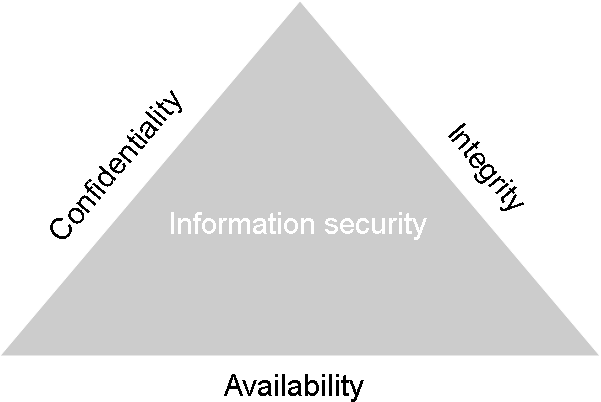
\includegraphics[width=10cm]{figures/cia.png}
	\caption{CIA triad}
	\label{fig:CIA triad}
\end{figure}


\subparagraph{Confidentiality}
Confidentiality is keeping information secret from unauthorized people. This is a major goal in information security. Encryption and access control are common ways of ensuring confidentiality \cite{michael2012}.

In a secure messaging system confidentiality would be guaranteed if the message being sent is only readable by the recipient and no one else \cite{sok}.

\subparagraph{Integrity}
Integrity is providing that information is unaltered and can only be changed by authorized people. If information is intercepted and changed during transit it would be a violation of integrity \cite{michael2012}.  
More specifically for a secure messaging it would mean that no altered message is accepted by the recipient \cite{sok}.

\subparagraph{Availability}
Making sure that information is accessible to authorized people is the goal of availability. Denial of Service attack \footnote{https://en.wikipedia.org/wiki/Denial-of-service\_attack} are common attacks targeting availability. 

Availability is generally more related to the system being available where the information itself plays a minor role \cite{michael2012}.
\\
\\
Depending on the type of system other properties must be satisfied as well. 


\subsection{Security properties}
The goal in a secure messaging system is to protect the messages being sent. The following properties are used to evaluate Matrix in section \ref{evaluationofmatrix}. 


\subparagraph{Authentication}
When a message is received the participant can verify that the message was sent from the actual sender. Furthermore a participant will receive evidence from a participant in a conversation that hey hold a known long-term secret. 



\subparagraph{Perfect Forward Secrecy}
If all keys are compromised than the decryption of any previously sent message should not be possible. Hence all previous messages would be secure however all future messages would be insecure 

\begin{figure}[H]
	\centering
	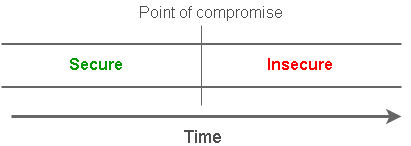
\includegraphics[width=10cm]{figures/forwardsecrecy.png}
	\caption{Forward secrecy}
	\label{fig:forward}
\end{figure}

\subparagraph{Backward secrecy}
If all keys are compromised than the decryption of \emph{future} messages should be possible. This property also goes by the names \emph{future secrecy} and \emph{post compromise security}. 

\begin{figure}[H]
	\centering
	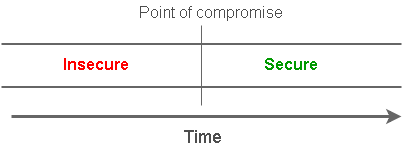
\includegraphics[width=10cm]{figures/backwardsecrecy.png}
	\caption{Backward secrecy}
	\label{fig:backward}
\end{figure}


\subsubsection{Other security properties}


\subparagraph{Participant Consistency} 
Whenever a message is accepted by a participant all participants are guaranteed to have identical view of the participant list.

\subparagraph{Destination Validation}
When a participant receives a message it can be verified that the participant was the intended recipient.

\subparagraph{Anonymity Preserving} 
The anonymity of the participants should be preserved and not linking any key identifiers.

\subparagraph{Speaker Consistency} 
There is consensus among the participants on the sequence of messages they receive by each participant. There might be a mechanism for checking consistency whenever a message is sent or after it has been received.

\subparagraph{Causality Preserving}
Messages must not be displayed before the message that originally precedes it has been displayed.

\subparagraph{Global Transcript} 
A global order where all messages are viewed in the same order for all participants.

\subparagraph{Deniability}
Deniability is a property where other participants cannot confirm that the message being sent was from the sender. Yet during the conversation there will be assurance for the recipient that the message being sent was authentic and sent by the sender \cite{sok}.

\begin{itemize}
	\item \emph{Message Unlinkability:} A deniability property that gives no guarantees that if a participant sent a message that other messages was sent by that participant as well. 
	\item \emph{Message Repudiation:} It can not be proved that a message was authored by a participant given the conversation transcript and all cryptographic key material. 
	\item \emph{Participant Repudiation:} It can not be proved that a participant was in a group conversation without his conversation transcript and cryptographic key material. 
\end{itemize}

The following properties are also defined in the paper \emph{SoK: Secure Messaging} but are less relevant for security.

\subparagraph{Group}

\begin{itemize}
	\item \emph{Computational Equality:} The computational load is equal for all participants.
	\item \emph{Trust Equality:} There is equal trust among all participants. 
	\item \emph{Subgroup messaging:} In the same conversation a participant can send messages to a subset of the participants.
	\item \emph{Contractible Membership:} When a participant leaves a conversation the protocol does not need to restart.
	\item \emph{Expandable Membership:} When a participant joins a conversation the protocol does not need to restart.
\end{itemize}

\subparagraph{Adoption}

\begin{itemize}
	\item \emph{Out-of-Order Resilient:} Messages received out-of-order should be accessible when received.
	\item \emph{Dropped Message Resilient:} On a unreliable network messages might be dropped in transit however it should not prevent decryption of future messages.
	\item \emph{Asynchronous:} Messages can be sent securely to recipients while they are offline.
	\item \emph{Multi-Device Support:} A participant can have multiple devices in a conversation and each device must be synchronized and should have the same historical conversation view
	\item \emph{No Additional Service:} There is no requirement of additional infrastructure being setup other than the participants. 
\end{itemize}




\section{Matrix}

Matrix is an open standard protocol for messaging over HTTP and synchronizing data. Matrix provides secure real-time communication over a decentralized federated network with eventual consistency. Matrix cover use cases such as instant messaging, VoIP, Internet of Things communication and is generally applicable anywhere for subscribing and publishing data over standard HTTP API.

%Any kind of json can be published to a room \cite{matrixvideoiot}.
% 3:10


% https://www.youtube.com/watch?v=-ofZMnKkp_Y 5:00 , 18:30

\subsection{How does it work?}

Matrix defines a conceptual place \emph{room} where data can be published and subscribed to. A room is shared and replicated among multiple \emph{homeservers}. The example shown in figure \ref{fig:matrix1} is a conversation in a room between three clients on different homeservers. 

In the example Alice starts by sending a message to the room. When Alice sends a message it is send to her homeserver. Each homeserver stores messages in a \emph{directed acyclic graph} called an \emph{event graph}. The message send by Alice is added to the event graph and is linked to most recent message(s) in the graph. The message is then signed with the signtatures of all previous messages by Alice's homeserver in order to make it tamper-proof. Finally the homeserver relays the message to the Bob's and Charlie's homeservers.

Upon receiving the message the other homeservers validates the message and then adds it to their own event graph. The message now persists in Bob's and Charlie's servers and can be retrieved from Bob's and Charlie's clients.

\begin{figure}[H]
	\centering
	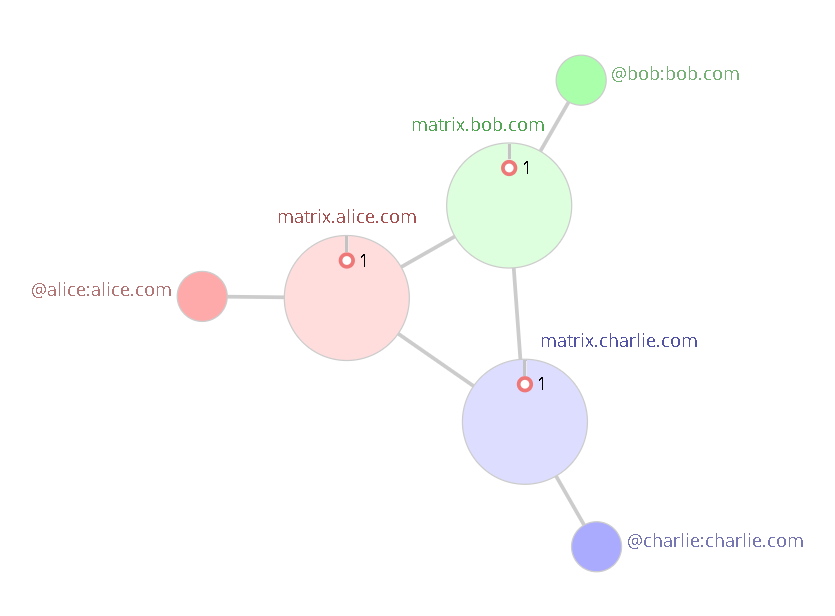
\includegraphics[width=9cm]{figures/matrix1.png}
	\caption{ Matrix \cite{matrixhome}.}
	\label{fig:matrix1}
\end{figure}

Bob replies to Alice's message and is first send to the homeserver and linked to Alice's message in the event graph. At the same time Charlie also send a reply and an inconsistency occurs as depicted in figure \ref{fig:matrix2}.


\begin{figure}[H]
	\centering
	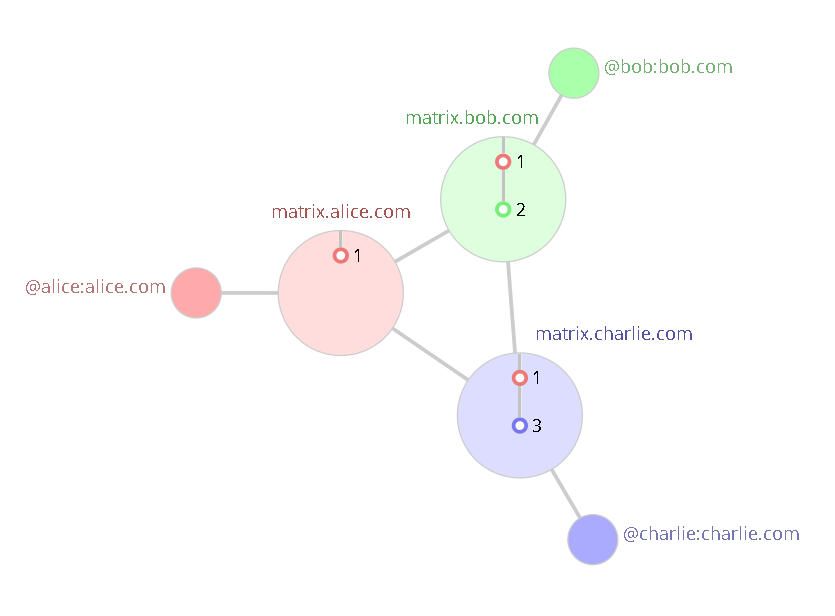
\includegraphics[width=9cm]{figures/matrix2.png}
	\caption{ Matrix \cite{matrixhome}.}
	\label{fig:matrix2}
\end{figure}


Bob's message arrives first to Alice and Charlie's homeservers. Alice adds the message to her own event graph and has a view that is consistent with Bob's. Charlie adds the message to the event graph; Bob's message precedes Alice's message hence message 2 and 3 are linked to message 1 shown in figure \ref{fig:matrix3};


\begin{figure}[H]
	\centering
	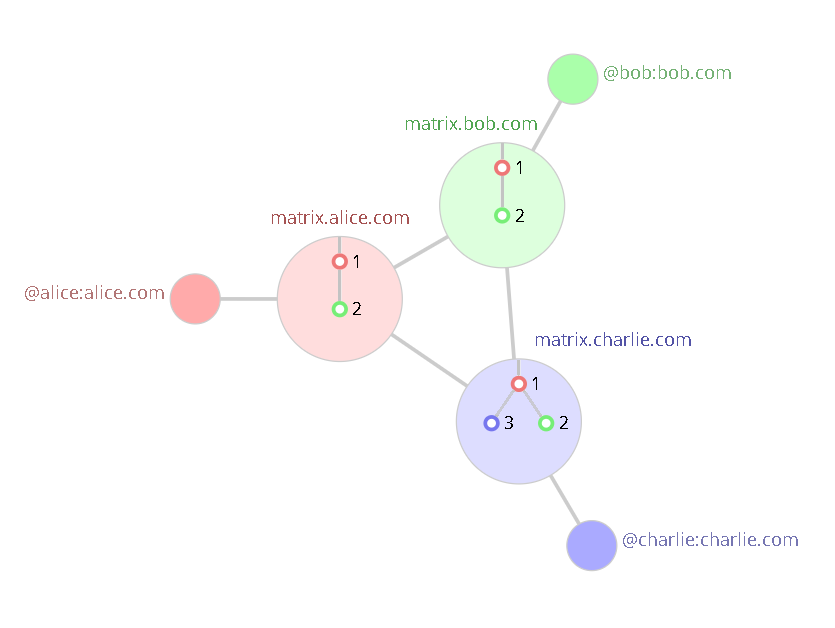
\includegraphics[width=9cm]{figures/matrix3.png}
	\caption{ Matrix \cite{matrixhome}.}
	\label{fig:matrix3}
\end{figure}


The other homeservers then receive Charlie's message and is added to their event graph. The room is yet again in sync and all the homeservers have a consistent view of the room.


\begin{figure}[H]
	\centering
	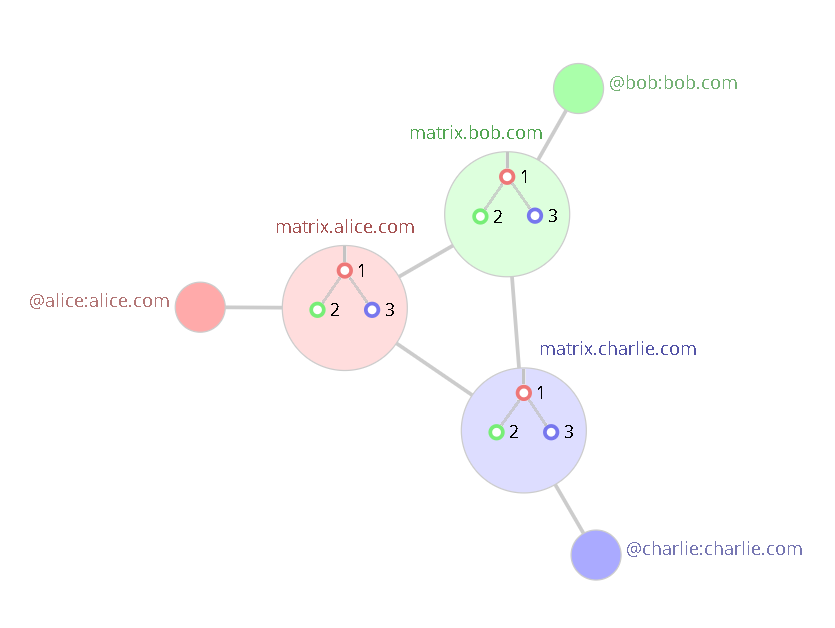
\includegraphics[width=9cm]{figures/matrix4.png}
	\caption{ Matrix \cite{matrixhome}.}
	\label{fig:matrix4}
\end{figure}

Alice sends a new message and is linked to the most recent unlinked objects (both Bob's and Charlie's). The message is then relayed to the other homeservers. The split in the event graph is merged. This example also shows how Matrix provides eventual consistency.

\begin{figure}[H]
	\centering
	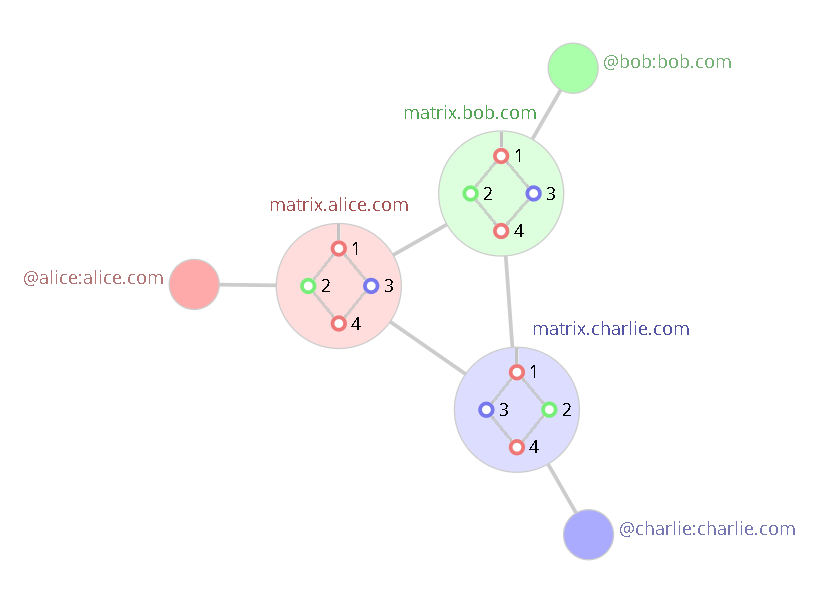
\includegraphics[width=9cm]{figures/matrix5.png}
	\caption{ Matrix \cite{matrixhome}.}
	\label{fig:matrix5}
\end{figure}

%In the example above the message is represnted by a JSON object and could be of any kind of object.


\subsection{Architecture} \label{matrix:architecture}
The previous section introduced the notion of a\emph{room} which clients sends messages to. The messages being in Matrix are actually JSON objects called \emph{events}. The events can be of any kind of structure hence it is not limited to messaging. Events are stored at homeservers and the communication history for a room is modelled using \emph{directed acyclic graph} called\emph{event graphs}. Matrix provides a specification for Client-Server API which is used for sending and synchronizing events between the client and its belonging homeserver. Matrix also provides specification for a Server-Server API which synchronizes data among homeservers with eventual consistency. The synchronization process between homeservers is defined by the term \emph{Federation} \cite{matrixspec}. 


\begin{figure}[H]
	\centering
	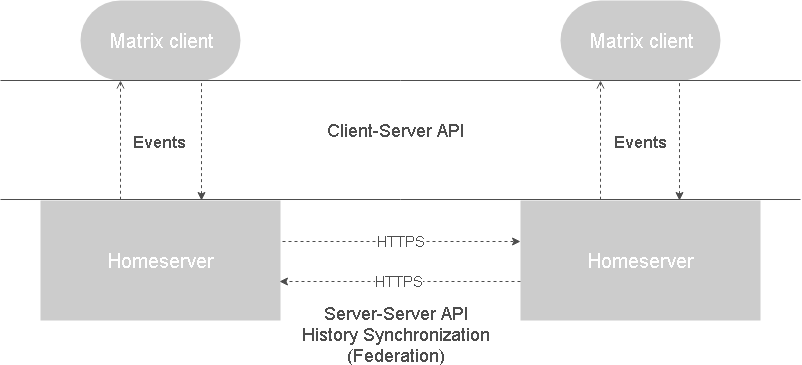
\includegraphics[width=11cm]{figures/matrix_architecture.png}
	\caption{ Matrix conceptual architecture \cite{matrixspec}.}
	\label{fig:matrix_architecture}
\end{figure}


As previously mentioned a room is a conceptual place for sending and receiving events with the room data being distributed over each homeserver. Each room is uniquely identified by a \emph{Room ID}. The figure \ref{fig:matrix_room} shows how events are send and received from a room.



\begin{figure}[H]
	\centering
	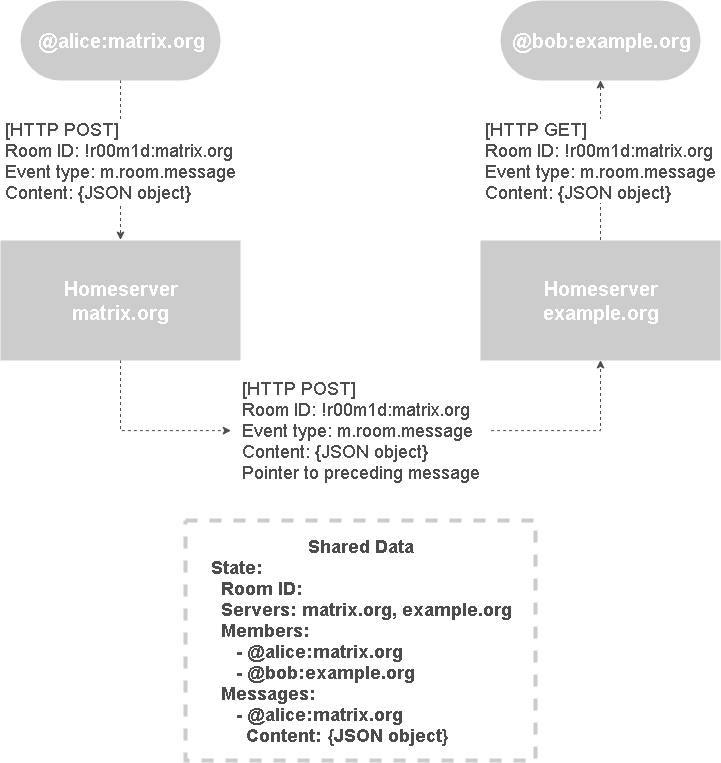
\includegraphics[width=10cm]{figures/matrix_room.png}
	\caption{ Matrix conceptual architecture \cite{matrixspec}.}
	\label{fig:matrix_room}
\end{figure}

\subsubsection{Event}

Every data exchange in Matrix is an event. Events are used to express state changes in a room as well as messages being sent. An event has a type used to differ between what kind of event is being sent and what kind of data it might hold. Matrix comes with reserved name spaces; \emph{m.room.message} is a type for instant messaging. The following is an example of a event of type \emph{m.room.message} \cite{matrixspec}.


\begin{lstlisting}[style=json]
{
	"content": {
		"body": "Hello world!",
		"msgtype": "m.text"
	},
	"room_id": "!wfgy43Sg4a:matrix.org",
	"sender": "@bob:matrix.org",
	"event_id": "$asfDuShaf7Gafaw:matrix.org",
	"type": "m.room.message"
}
\end{lstlisting}

The specification is open for defining custom types which can express any kind of data one might want to exchange \cite{typeofevent}.


\subsection{Matrix specification}
Matrix has two main API specifications; Client/Server API and Federated API. Any Matrix SDK implements the API defined at the Client/Server API specification. If a custom homeserver was to be developed from scratch it would have to conform to the Federated API to be able to be a part of Matrix. 

\subparagraph{Client/Server API}
For clients to send and receive messages the Client/Server API is used. The API mainly provides specification for:

\begin{itemize}
	\item Sending and receiving messages
	\item Configure rooms
	\item Synchronize historical conversation
\end{itemize}

There exist several SDKs implementing the API.  

\subsection{End-to-end Encryption}
Security is a high priority for Matrix design. Especially with the decentralized architecture with data being replicated over a federation federation of servers. Matrix provides security guarantees through end-to-end encryption using Olm and Megolm cryptographic ratchet. Olm is based on the Double Ratchet algorithm and Megolm is an extension for secure group communication. Olm and Megolm are examined in section \ref{matrixeval}.



\subsection{Concepts}



\subsubsection{Diffie-Hellman Key Exchange}

Diffie-Hellman is a key exchange protocol to establish a shared secret over an insecure channel. Public information is send over an insecure and using asymmetric keys two parties can derive the same shared key.


The first step is to agree on some public values. Either of the parties start the protocol by picking a large prime \emph{p} and a integer \emph{g} then the values are sent over the insecure channel.  

\begin{figure}[H]
	\hspace*{-1cm} 
	\centering
	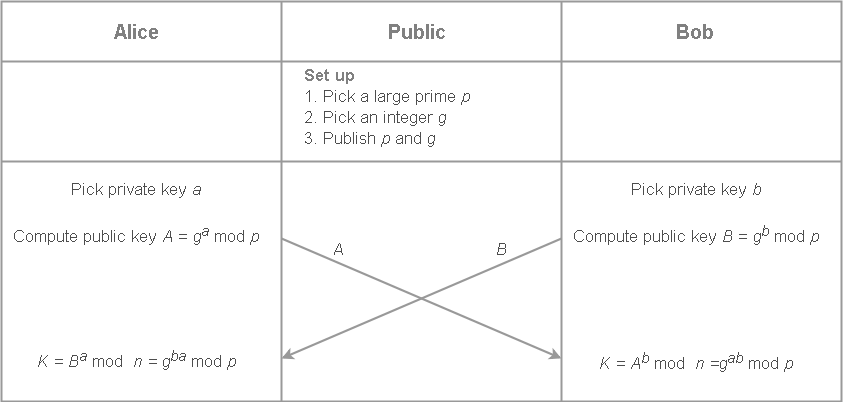
\includegraphics[width=14cm]{figures/dh.png}
	\caption{Simple Diffie-Hellman Key Exchange}
	\label{fig:dh}
\end{figure}

Alice and Bob will each pick a private key value and compute a public key value. The computed key value is sent over the insecure channel and Alice and Bob will both perform the same computation as previously \cite{crypto101}.


The Diffie-Hellman is vulnerable to man in the middle attack since there is no authentication taking place. There exist a solution to this problem using asymmetric key pairs and signing the messages being sent \cite{crypto101}.

\subsubsection{Key Derivation function}

Assume a secret key is established between two parties and is used to encrypt messages and exchange them over an insecure channel. An adversary listening might store all the messages being send even though he is not able to read them. However at some point he manages to compromise the secret key hence being able to decrypting every message ever sent.

To overcome the above scenario ephemeral keys are used. Such keys are short lived and are discarded after use.   

New secret keys can be generated using a \emph{Key Derivation Function} (KDF).
A KDF is a one way function that derives one or more randomized secret keys based on a secret key (or multuple) and optionally some input value \cite{crypto101}. Figure \ref{fig:kdf} illustrates this.

\begin{figure}[H] 
	\centering
	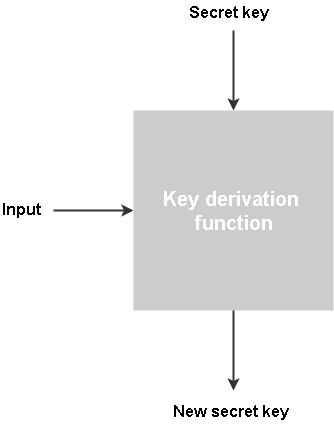
\includegraphics[width=8cm]{figures/kdf.png}
	\caption{Key derivation function}
	\label{fig:kdf}
\end{figure}


A core concept in the Double Ratchet algorithm is KDF chains which build a chain of secret keys using KDF \cite{doubleratchet}. 


\subsubsection{Signal Protocol}

The Signal Protocol provides end-to-end encryption and was developed in 2013 and was first introduced in the app TextSecure\footnote{https://en.wikipedia.org/wiki/TextSecure}.

The Signal Protocol consists of two parts; The \emph{Triple Diffie-Hellman protocol} (TripleDH) and the Double Ratchet algorithm.

\paragraph{Triple Diffie-Hellman protocol}\label{tripledh}
Before the Double Ratchet algorithm can be used the two parties communicating need to agree on a shared secret key. In the Signal protocol this is achieved with Triple Diffie-Hellman protocol \emph{(TripleDH)}.

The Triple Diffie-Hellman protocol is a \emph{key agreement protocol}. It involves a server and two parties; Alice and Bob. 

The TripleDH protocol is characterized by three phases:

\begin{enumerate}
	\item \emph{Publishing keys:} A identity key and several prekeys belonging to Bob is published by him to a server.
	\item \emph{Sending initial message:} Alice sends an initial message to Bob. A prekey bundle is obtained by Alice from the server in order to send an initial message to Bob.
	\item \emph{Receiving initial message:} Alice's message is received and processed by Bob.
\end{enumerate}


\paragraph{Double Ratchet algorithm}

After a shared secret key has been established the Double Ratchet algorithm can then be used to send and receive encrypted messages.

Each party has three chains; root chain, sender chain and receive chain. The chains are KDF chains and will take two keys as input (a KDF chain key and some other input key) and output new two keys (a new KDF chain key and some other output key). The KDF chain is illustrated in figure \ref{symkeyratchet}.

The algorithm has a \emph{Diffie-Hellman ratchet} step and \emph{symmetric ratchet} step and the chains are used across both steps.

\begin{itemize}
	\item \emph{Diffie-Hellman ratchet:} The parties exchanges new Diffie-Hellman public keys with the messages being sent. New secrets are then derived using Diffie-Hellman (DH). The secret that DH outputs is used as input to the root chain. The root chain then output new chain keys for the receiving and sending chains. 
	
	\item \emph{Symmetric ratchet:} The sending and receiving chains uses the chain keys derived from the root chain and for each message sent and received the chains are advanced. The output from the receiving and sending chains are keys for encrypting or decrypting messages. 
\end{itemize}


\subparagraph{Symmetric ratchet}
The symmetric ratchet provides message key through the receiving and sending chains. A message key is used for encryption or decryption of a message.

In the symmetric ratchet a single ratchet step is the calculation of the next key chain and message key. The inputs are the current chain key and a constant. Figure \ref{fig:symkeyratchet} illustrates two steps in a symmetric ratchet.

\emph{Forward secrecy} is provided since KDF is a one-way function and it is not possible to go backward and get the input chain key from the output chain key. However since the other input is simply a constant all future keys chain keys and message keys can be derived from an older chain key more specifically there is lack of backward secrecy.


\begin{figure}[H]
	\centering
	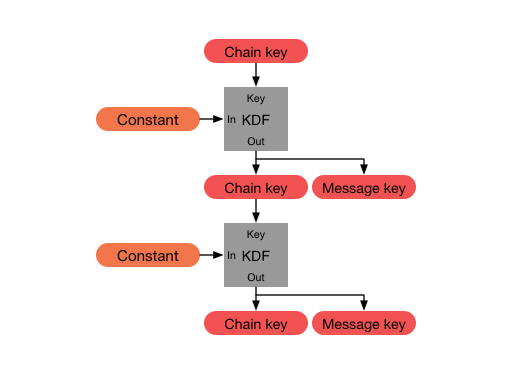
\includegraphics[width=10cm]{figures/symmetrickeyratchet.png}
	\caption{Symmetric key ratchet \cite{doubleratchet}.}
	\label{fig:symkeyratchet}
\end{figure}


\newpage
\subparagraph{Diffie-Hellman ratchet}

Double ratchet provides backward secrecy by comining the Symmetric ratchet with a Diffie-Hellman ratchet hence the name \emph{Double Ratchet}.

Every message from either party begins with a header which contains the sender's current ratchet public key. Whenever a new ratchet public key is received a new ratchet key pair is generated; a secret is derived through Diffie-Hellman with the input being the received ratchet public key and the ratchet private key from the new generated key pair.

Alice starts a conversation with Bob and uses his published public key as a ratchet public key. Alice then generates a new ratchet key pair and derives a shared secret key using Diffie-Hellman and would that as input to her \emph{sending chain}. Alice then sends her new ratchet public key to Bob. At the receiving end Bob derives the same shared secret which would be the input to his \emph{receiving chain}. Alice's sending chain and Bob's receiving chain share the same secret hence he can derive the message key and decrypt the message sent from Alice. When Bob sends a reply to Alice he would generate a new ratchet key pair and derive a new secret which would be input to his \emph{sending chain}.

Figure \ref{fig:dhratchet1} shows an ongoing message exchange with new secrets being derived and the sending and receiving chains being advanced.

\begin{figure}[H]
	\centering
	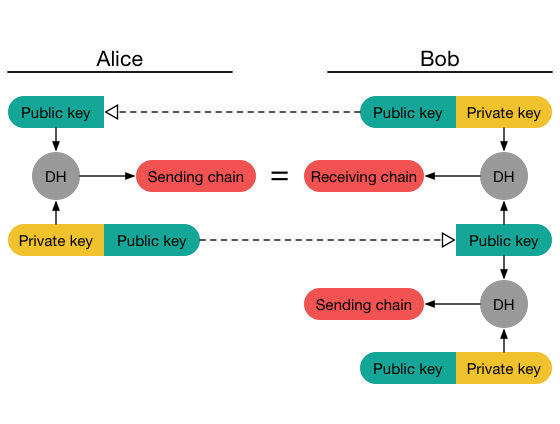
\includegraphics[width=9cm]{figures/dhratchet5.png}
	\caption{Diffie-Hellman ratchet \cite{doubleratchet}.}
	\label{fig:dhratchet1}
\end{figure}


When Alice receive the reply from Bob she would perform the exact same steps. This ultimately results in a continous loop of generating new ratchet key pairs and using Diffie-Hellman to derive the same shared secret key. A continuation is shown in figure \ref{fig:dhratchet2}

\begin{figure}[H]
	\centering
	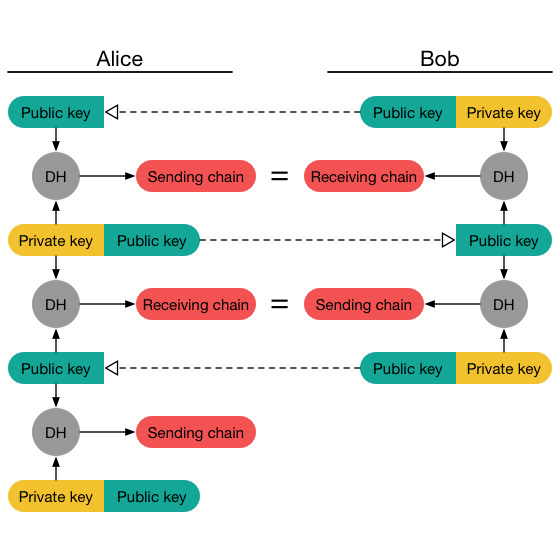
\includegraphics[width=9cm]{figures/dhratchet6.png}
	\caption{Continuation of Diffie-Hellman ratchet  \cite{doubleratchet}.}
	\label{fig:dhratchet2}
\end{figure}


As mentioned in the beginning of the Double Ratchet section the Diffie-Hellman ratchet does have a root chain which would provide inputs to the sending and receiving chains. A more correct view of the process in Diffie-Hellman is shown in figure \ref{fig:dhratchetcon}. 


\begin{figure}[H]
	\centering
	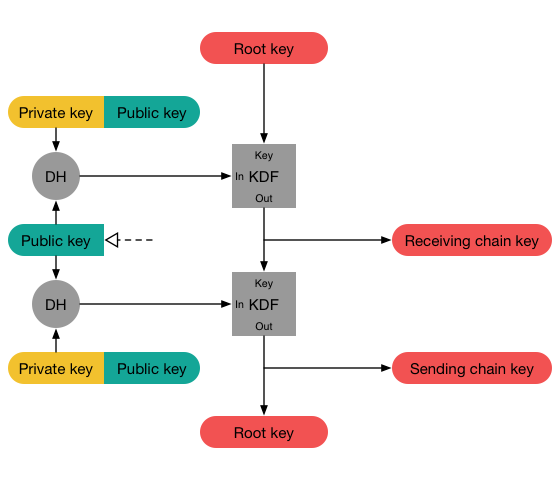
\includegraphics[width=9cm]{figures/dhratchet7.png}
	\caption{Diffie-Hellman ratchet 7 \cite{doubleratchet}.}
	\label{fig:dhratchetcon}
\end{figure}

\paragraph{Double ratchet}

When combining Diffie-Hellman ratchet and symmetric-key ratchet the result is the Double ratchet.

\begin{itemize}
	\item When sending or receiving a message the corresponding message key is derived by performing a symmetric-key ratchet step.
	\item Upon receiving a new ratchet public key the Diffie-Hellman ratchet step performed right before the symmetric-key ratchet step with the goal of replacing old chain keys with new ones.  
\end{itemize}

Assume that the message exchanged is a continuation from the TripleDH key exchange described in section \ref{tripledh}. Alice had sent an initial message. The initial ratchet public key would be Bob's signed prekey \emph{SPK\textsubscript{B}} and the new ratchet key pair would be the Alice's ephemeral key pair that she generated. Alice calculated a shared secret which is the \emph{root key}. She then generates a new ratchet key pair and takes the output from Diffie-Hellman and use it as input for the \emph{root chain}. The root chain then outputs a new root key \emph{RK} and a sending chain key {CK}.

The figure \ref{doubleratchet1} depicts this with a view of Alice's chains.


\begin{figure}[H]
	\centering
	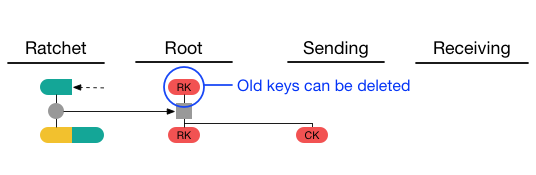
\includegraphics[width=10cm]{figures/doubleratchet1.png}
	\caption{Double ratchet 1 \cite{doubleratchet}.}
	\label{fig:doubleratchet1}
\end{figure}

When Alice then sends a message \emph{A1} the symmetric-key ratchet step will return a new chain key and a message key. The message can then be encrypted with the message key.

\begin{figure}[H]
	\centering
	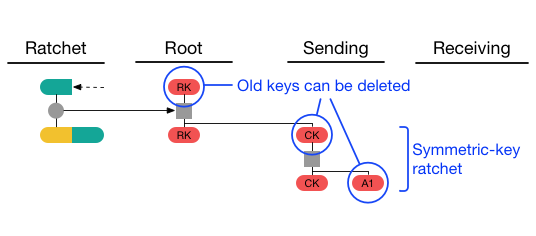
\includegraphics[width=10cm]{figures/doubleratchet2.png}
	\caption{Double ratchet 2 \cite{doubleratchet}.}
	\label{fig:doubleratchet2}
\end{figure}

Next Alice receives a message \emph{B1} from Bob. The message header contains a new ratchet public key and a Diffie-Hellman ratchet step is performed. New sending and receiving chain keys are derived and followed by a symmetric-key ratchet step to derive the receiving message key to decrypt the message.

\begin{figure}[H]
	\centering
	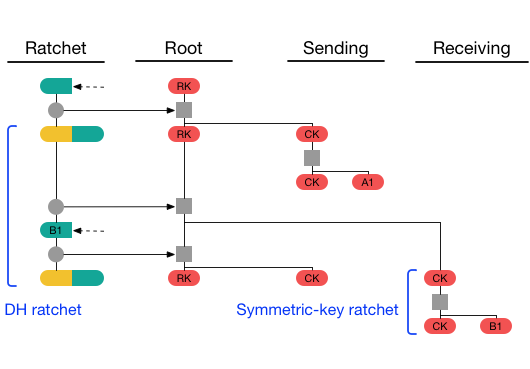
\includegraphics[width=10cm]{figures/doubleratchet3.png}
	\caption{Double ratchet 3 \cite{doubleratchet}.}
	\label{fig:doubleratchet3}
\end{figure}






% This chapter will present the criteria \emph{evaluation of Matrix security model}

\section{Evaluation of Matrix security model}\label{evaluationofmatrix}
The security of matrix will be evaluated in the context of secure messaging. An evaluation framework has been proposed in the paper \emph{SoK: Secure messaging} which the evaluation will be loosely based on. 

The evaluation framework covers several areas with \emph{conversation security} being the most relevant for this evaluation. The area \emph{conversation security} describes three categories; \emph{Security and Privacy}, \emph{Adoption}, and \emph{Group Chat}. Obviously the most relevant category for the evaluation is \emph{Security and Privacy}

\subsection{Threat model}
For secure messaging the evaluation framework defines a threat model with three types of adversaries. Note that an adversary can be of several types:

\begin{itemize}
	\item \emph{Local adversary:} The adversary is in control of the local network.
	\item \emph{Global adversary:} The adversary is in control of great portions of the Internet 
	\item \emph{Service providers:} A potential adversary for messaging systems with centralized infrastructure.
\end{itemize}

In the messaging system the adversary may be a participant with the following properties:

\begin{itemize}
	\item An adversary can start a conversation.
	\item An adversary can send messages.
	\item An adversary can perform any other action that a participant is capable of.
\end{itemize}

Furthermore it is assumed that the system's endpoints are secure \cite{sok}.

This evaluation will inherit the described threat model.

\subsection{The Signal Protocol}
Matrix provides end-to-end encryption by using the Olm and Megolm library with the former being an implementation of the Double Ratchet algorithm also known as the Signal Protocol, and the latter being the algorithm used for group chat. 

Olm is used for securely exchanging message keys/session keys during group chat and is vital part of the end-to-end encryption in Matrix.

Before the Matrix protocol is evaluated the Signal Protocol will be considered. The Signal Protocol is described in section xx. 

Section xx provides a list of security properties relevant for \emph{conversation security}. These security properties is used for evaluating a secure messaging protocol such as the Signal Protocol.
%Any messaging application that provides end-to-end encryption is likely an implementation of  the protocol 

The table below shows an evaluation of the Signal Protocol (previously known as TextSecure) \cite{sok}. 

\begin{figure}[H]
	\hspace*{-1.7cm} 
	\centering
	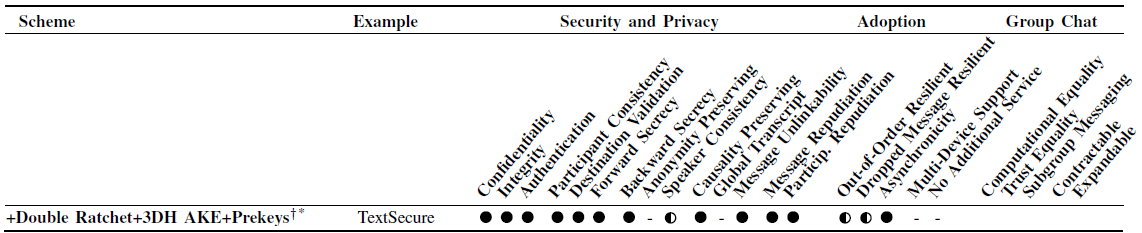
\includegraphics[width=16cm]{figures/framework_signal.png}
	\caption{Evaluation of Signal (TextSecure) \cite{sok}.}
	\label{fig:framework_signal}
\end{figure}


%Explain how they provide the properties or why they don't


\subparagraph{Confidentiality} When a message is sent using the Signal Protocol then only the intended recipient can read the message. The senders sending ratchet and receivers receiving ratchet will derive the same message key hence only the two parties will be able to encrypt the messages. 

\subparagraph{Integrity} The receiver will only accept a message if it is successfully decrypted hence if in transit a message was modified then the message would be rejected.

\subparagraph{Authentication} The decryption of a message also gives authentication guarantees since only the intended recipient could compute the message key.

\subparagraph{Forward secrecy} The symmetric ratchet ensures forward secrecy. If a chain session key is compromised then the previous keys can not be generated since the ratchet is one way cryptographic hash function hence secrecy is provided for all previous send messages.  

\subparagraph{Backward secrecy} Diffie-Hellman ratchet have the self-healing property and will generate a new chain session key for the symmetric ratchet hence if a chain key is compromised then secrecy for future messages is still provided because a new chain ratchet key will be generated.

\subparagraph{Anonymity preserving}

Anonymity preservation is lost in the Signal Protocol since the initial key agreement requires long-term public keys hence making them observable during Triple-DH. However \textbf{\emph{participant consistency}} is provided by Triple-DH \cite{sok}. %How?
%Without participant consistency, identity misbinding attacks might be possible. Unknown key share attack

\subparagraph{Speaker consistency}
This property is partially provided through the key evolution of the ratchets. If a message is dropped then it is not possible to generate message keys for future messages. This also makes the protocol have the property \textbf{\emph{Causality Preserving}} and partially have the property \emph{\textbf{Dropped message resilence}}. It will also not go unnoticed if a message is received out of order since this will result in the message's key being an unexpected key. Hence the recipient have to store expired keys to decrypt delayed messages. This makes the property \emph{\textbf{Out-of-order resilient}} only partially provided \cite{sok}.

\subparagraph{Global transcript} 
In an asynchrounous messaging protocol there is no global transcript. Both participants have to be online to receive messages hence the participants will not have all the messages if one of them is offline. This is a result of having the \textbf{\emph{Asynchronicity}} property.

\subparagraph{Deniability properties}

Since the ratchet session keys are used for encrypting messages and not the long-term public keys the properties \textbf{\emph{Message unlinkability}} and \textbf{\emph{Message repudiation}} are provided. 


\subparagraph{Other properties}

\begin{itemize}
	\item \textbf{\emph{Participant repudiation}}. Triple-DH achieves full participant repudiation since anyone can forge a transcript between any two participants \cite{sok}.
	\item \textbf{\emph{Destination validation}}. The Deffie-Hellman ratchet provides this property since the recipients public key is used to generate the chain key \cite{sok}. % Is this true?
\end{itemize}


The evaluation shows that several security properties are provided with the important ones being confidentiality, integrity, authentication, forward secrecy, backward secrecy. 

Furthermore a formal analysis have been made on the Signal Protocol that proves the protocol is free from any major flaws and it satisfy the following security properties; confidentiality, authentication and secrecy \cite{Signal}. 

\paragraph{Application variants}

The Signal Protocol is a secure messaging protocol and have been extensively studied including proof that the standard security properties are assured. 

The Olm library used by Matrix is a variant of the Signal Protocol. There is no implementation analysis of the Olm library hence there is no guarantee that all the security properties defined in xx is inherited by Olm. Nevertheless it is assumed that Olm inherits the above properties.

The further evaluation relies upon the the security assessment of Matrix. 


\subsection{Matrix protocol}\label{matrixeval}

As described in section xx \emph{rooms} are a fundamental part of Matrix' architecture. There can be multiple participants in a room hence the support for secure group conversation is required. 

Olm (and the Signal Protocol it is based on) is ideally meant for two party communication.
Group conversation could be supported with a näive variant of Olm. In a group with N participants each participant would establish a secure Olm session with every other participant. When a message is send each message would then have to be encrypted N times. This solution would scale poorly if N was a large number. This was the motivation for introducing Megolm.

\paragraph{Megolm}

Megolm is a multicast encryption solution \cite{sok}.Each sender has a sender ratchet (Megolm Ratchet). Each recipient has a corresponding receiving ratchet for each sender. So if there are N participants in a group then each participant will have N-1 receiving ratchets. Figure \ref{fig:megolm} illustrates the setup with three participants. 

\begin{figure}[H]
	\hspace*{-1cm} 
	\centering
	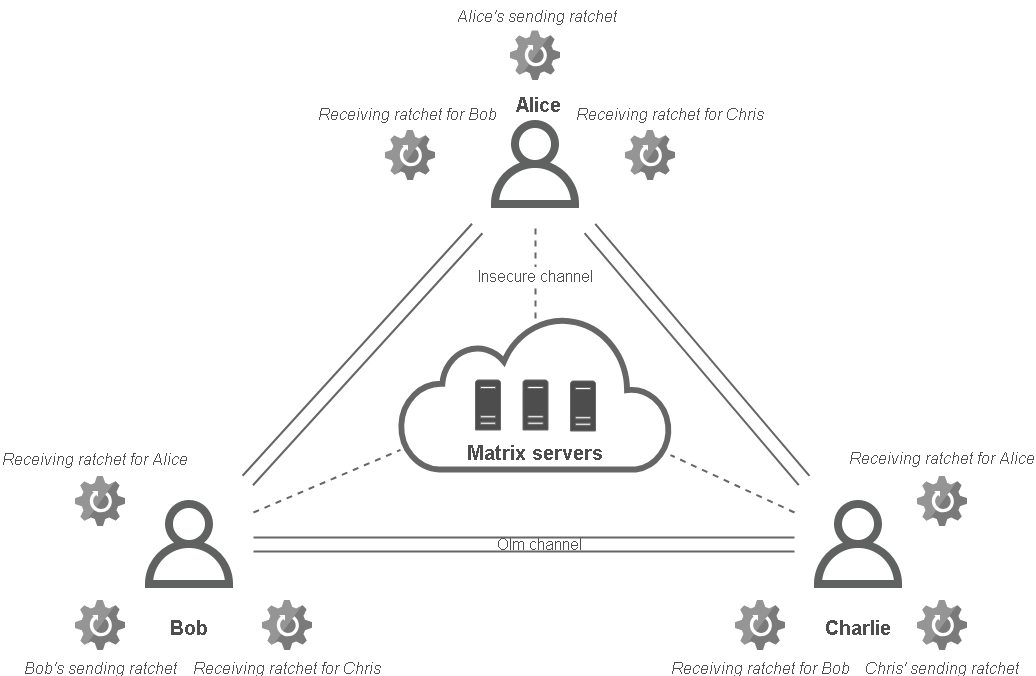
\includegraphics[width=14cm]{figures/megolm_conceptual.png}
	\caption{Conceptual model of Megolm with three participants.}
	\label{fig:megolm}
\end{figure}

When a session is started a sender will send his initial ratchet key to each recipient, so that the sender ratchet and each recipients ratchet are in sync. This key exchange happens over a secure communication channel (Olm). Furthermore there is send N-1 initial messages when a session is initiated. Until a new session is started no further session keys are exchanged and the corresponding message keys are generated by incrementing the ratchet.

When a sender sends a message a message key is generated from the ratchet key and the message is encrypted using that message key. The message will be signed so the recipient will know which sender the message is from and which ratchet to utilize. %(not with a long-term I guess? hence providing deniability)
The message  is then send to the server which relays the message to all recipients over an insecure channel. When they receive the message the same message key is generated using the corresponding receiver ratchet and the message is decrypted. 

When a new participant joins the latest ratchet key would then be shared by each participant over Olm (or an earlier one if he should have access to historical conversation). 

When a participant leaves a new session would be initiated yielding in refreshing the ratchet keys hence not making it possible for that ex-participant to decrypt any further messages.




% add figures for naive olm and multicast encryption solution

The Matrix Protocol will be evaluated in the context of Megolm. The evaluation of the Matrix protocol heavily relies on the security assessment by NCC.


\subsubsection{Evaluation}

The Matrix Protocol provides several security properties shown in the table xx. 

It is worth mentioning that there is a trade-off between security and usability which must be decided at application layer. The most secure configuration would come at the cost of usability and performance.    
\begin{itemize}
	\item \emph{Usability}. From a users point of view it would be nice to have the possibility to load historical conversation instead of having to keep full history locally. Matrix supports multiple devices and if a participant adds another device at some later point it makes sense to load the participants historical conversation into the device. From a security perspective this would mean that the \emph{initial ratchet state} is stored and is send to the new device so every message key can be generated. This certainly goes against the principle of forward secrecy. The most secure configuration would not store the \emph{initial ratchet state} hence satisfy forward secrecy thus disable the described usability feature \cite{ncc} \cite{megolm}.
	\item \emph{Performance}. When a megolm session is initialized there is an initial burst of messages to exchange the initial ratchet key which is then stored in a \emph{initial ratchet state} value at each recipient. If this key is compromised then any future key can be generated for that session. To satisfy backward secrecy this would mean initiating a new session for each message which would trigger a burst of messages to exchange the ratchet key \cite{ncc} \cite{megolm}. This would scale poorly for a large group or when sending large-sized messages. 
\end{itemize} 


\begin{figure}[H]
	\hspace*{-1.7cm} 
	\centering
	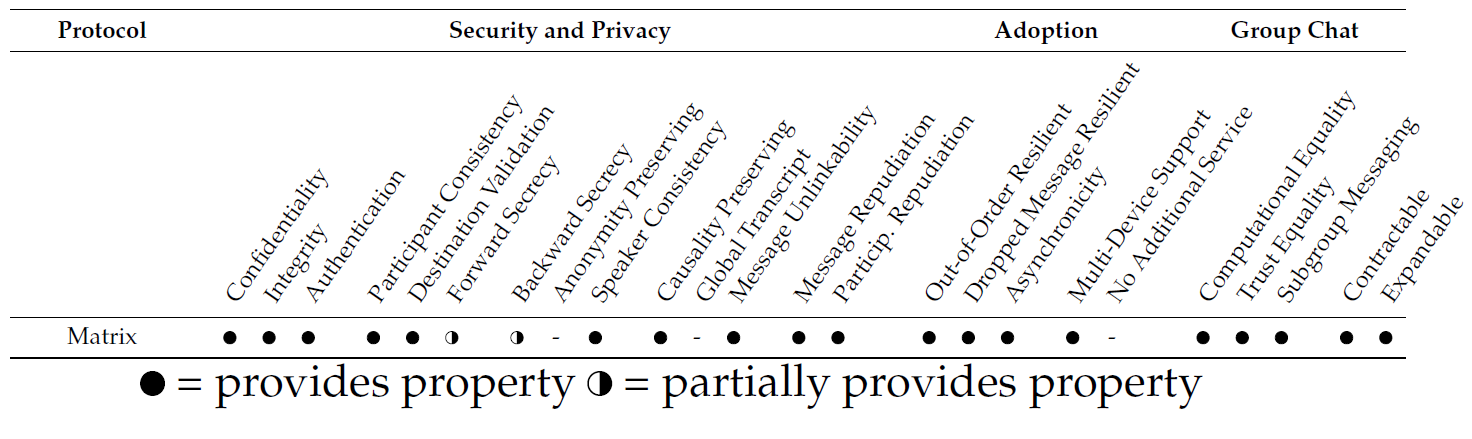
\includegraphics[width=16cm]{figures/framework.png}
	\caption{Evaluation of Matrix Security.}
	\label{fig:framework}
\end{figure}

Some of the security properties in the table are briefly examined.

\subparagraph{Confidentiality} When a message is send it is encrypted and can only be decrypted by the intended recipients who has the corresponding ratchet session key received over an Olm channel. 

\subparagraph{Integrity} The receiver will only accept a message if it is successfully decrypted hence if in transit a message was modified then the message would be rejected. 


\subparagraph{Forward secrecy} Each participant keeps a \emph{initial ratchet state} which holds the earliest ratchet session key for a session. This clearly violates forward secrecy since every message can be decrypted if the \emph{initial ratchet state} value is compromised. However it is a deliberate trade-off for usability to enable historical conversation and storing the value is optional. Since this is an optional feature the forward secrecy is partially provided \cite{ncc}. 

%From NCC

\subparagraph{Backward secrecy} If a ratchet key is compromised then an adversary can generate every message key from that point on hence intercept any message that sender sends to the group. This can be prevented strictly by starting a new session with every send message however it would not be possible to keep conversation history (only locally when data is encrypted). Hence the property is only partially provided \cite{ncc}.

% From NCC


\subparagraph{Speaker consistency}

There is no guarantee for speaker consistency. A well known problem of multi-cast encryption group chat is transcript inconsistency. A sender may send different messages to different recipients. However it requires that the server is in collusion with the sender. This also applies to \emph{\textbf{Causality preserving}} \cite{ncc}.


\paragraph{Other properties}

The multi-cast encryption design does not provide \emph{participant consistency} \cite{sok}.

The properties \emph{Dropped message resilence} and \emph{Out-of-order resilient} are provided by keeping track of ratchet indices. 

Several properties are inherited from the secure key exchanging channel provided by Olm while other properties are inherited because of asynchronicity of the Megolm protocol.

\begin{itemize}
	
	\item \emph{Authentication} is provided by Olm since the ratchet session key is send to the recipient through an Olm channel or else the message key could not be derived.
	\item \emph{Destination validation}. The ratchet session key is exchanged over a secure Olm channel hence only the intended recipient could decrypt it.
	\item \emph{Anonymity preserving} is not provided since Olm requires the long-term public key in the initial key exchange.
	\item \emph{Global transcript} is also not provided because of the asynchronous nature of the Megolm protocol.  
	\item \emph{Asynchronicity} is obviously provided.
	\item \emph{Deniability} properties are inherited from Olm as well.
\end{itemize}

All properties related to group chat are also provided. Although they are additional features and not related to security. 


\paragraph{Other findings}

\subparagraph{Message Replays}

Matrix allows decryption of a message multiple times hence it is vulnerable to replay attacks. Replay attacks are handled at the application layer. Whenever a message is decrypted a message index is generated and stored. If the exact message is decrypted again the same message index will be generated and can be compared to the stored message index making the replayed message invalid. 

\subparagraph{Unknown key-share attack}

The \emph{Unknown key-share attack}\footnote{https://en.wikipedia.org/wiki/Unknown\_key-share\_attack} is a vulnerability found with a high risk in Megolm. The vulnerability is inherited from Olm and occurs after the initial message in Triple-DH. 

The vulnerability has been mitigated at the application layer by providing a unique identifier for the sender and receiver into each message and then checking the values when decrypted \cite{ncc}.

\paragraph{Recent research}
The way backward secrecy would be provided in Matrix is computationally expensive. Recent research has proposed solutions with early implementations for these problems with IETF leading the research on the standard on \emph{Messaging Layer Security}. Matrix has expressed awareness of the protocol and a possibility of adaption in the future.

\subsection{End-to-end security} \label{endtoend}

Section xx describes Matrix long-term goal as being a generic HTTP messaging API. It could be utilized for any kind of data exchange in a system or between multiple systems.

A system using the Matrix Protocol for exchanging data would benefit from the security properties found in the evaluation yet the system-wide security or end-to-end security would be incomplete an further measures must be taken. Such system might demand confidentiality and integrity throughout the system yet the system as a whole would have a different threat model than the one described for a secure messaging system hence no guarantee of confidentiality or integrity beyond the endpoints in end-to-end encryption. 

The following figure depicts how end-to-end encryption might be inadequate in such system. 

\begin{figure}[H]
	\centering
	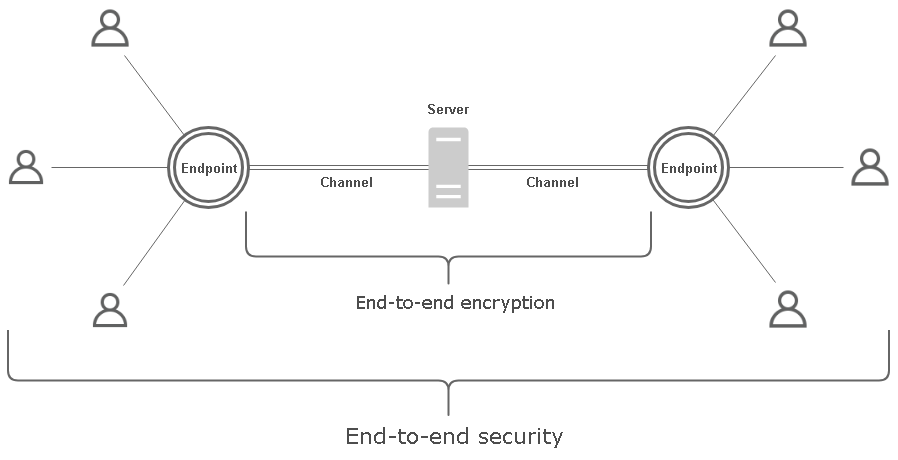
\includegraphics[width=12cm]{figures/e2esecurity.png}
	\caption{End-to-end security.}
	\label{fig:e2esecurity}
\end{figure}

As the system depicts there might be several principals accessing the endpoint. Each principal could retrieve some information possibly protected with access control. Assume that the information resting at the endpoint is of confidential nature; access could still be granted with no respect of the confidentially of that information. There clearly lack a mechanism of specifying what information is confidential or public and where it may flow under what conditions.  

\subparagraph{Matrix IoT}
Matrix identifies IoT as another use case. A person can have several devices for health tracking, entertainment and so on. The data from the devices are send to vendors - a device might send data to several vendors. Ultimately this give a fragmentation of the person's own data with it being placed at several vendors data back-end. Matrix proposes a solution where all the device data for a person is synchronized and persisted on Matrix. Vendors would be connected to Matrix. This is depicted in figure \ref{fig:matrix_iot} below. 

\begin{figure}[H]
	\centering
	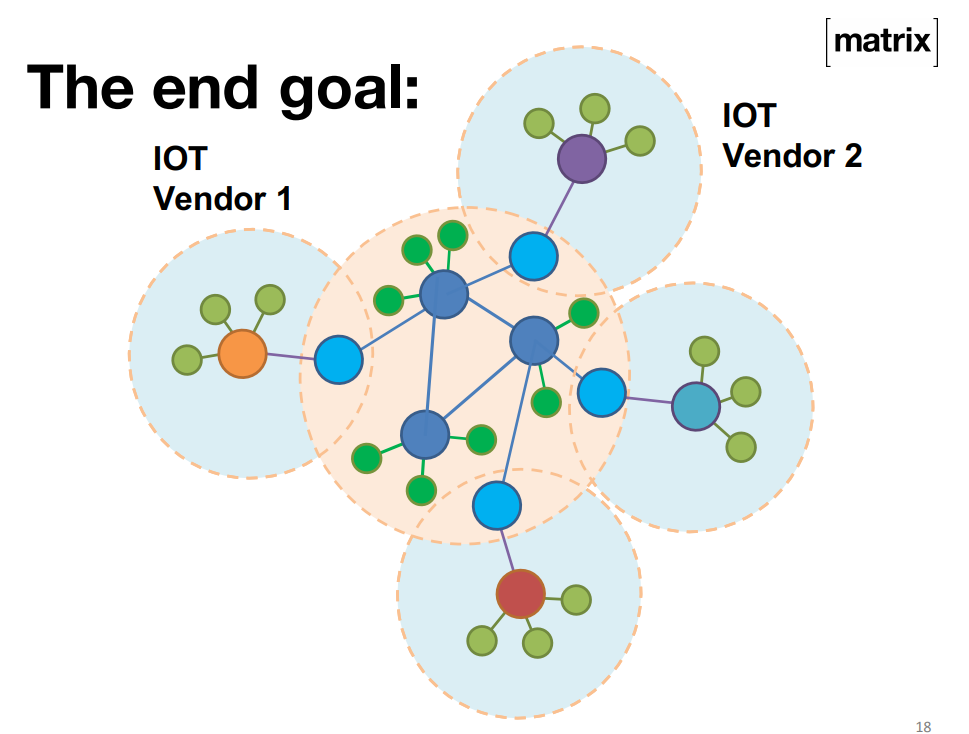
\includegraphics[width=10cm]{figures/matrix_iot.png}
	\caption{End goal for Matrix IoT}
	\label{fig:matrix_iot}
\end{figure}

The data flowing from the sensors to Matrix might be of sensitive nature or the owner might only allow some data to flow to some vendors under specific conditions. This issue related to confidentiality is not addressed by Matrix. 

\subsection{Evaluation summary}

In this section an evaluation of Matrix security was presented. Several security properties are a part of Matrix security model with forward secrecy and backward secrecy being provided depending on the Matrix configuration.

End-to-end encryption is not the end of security. Other security measures must be taken to provide confidentiality and integrity. Information Flow Control is such measure and the next section will present a survey on Information Flow Control.


